%%%%\Transcb{yellow}{blue}{De IceCube Neutrino Telescoop}
\Tr
\onecolumn
\begin{center}
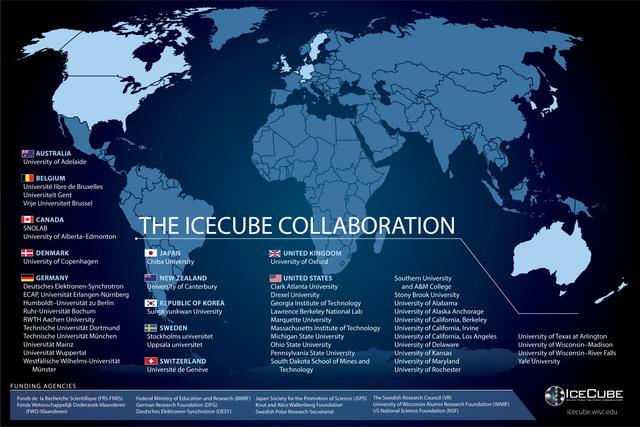
\includegraphics[keepaspectratio,height=15cm]{icecube-collab2}
\end{center}

\Tr
\begin{center}
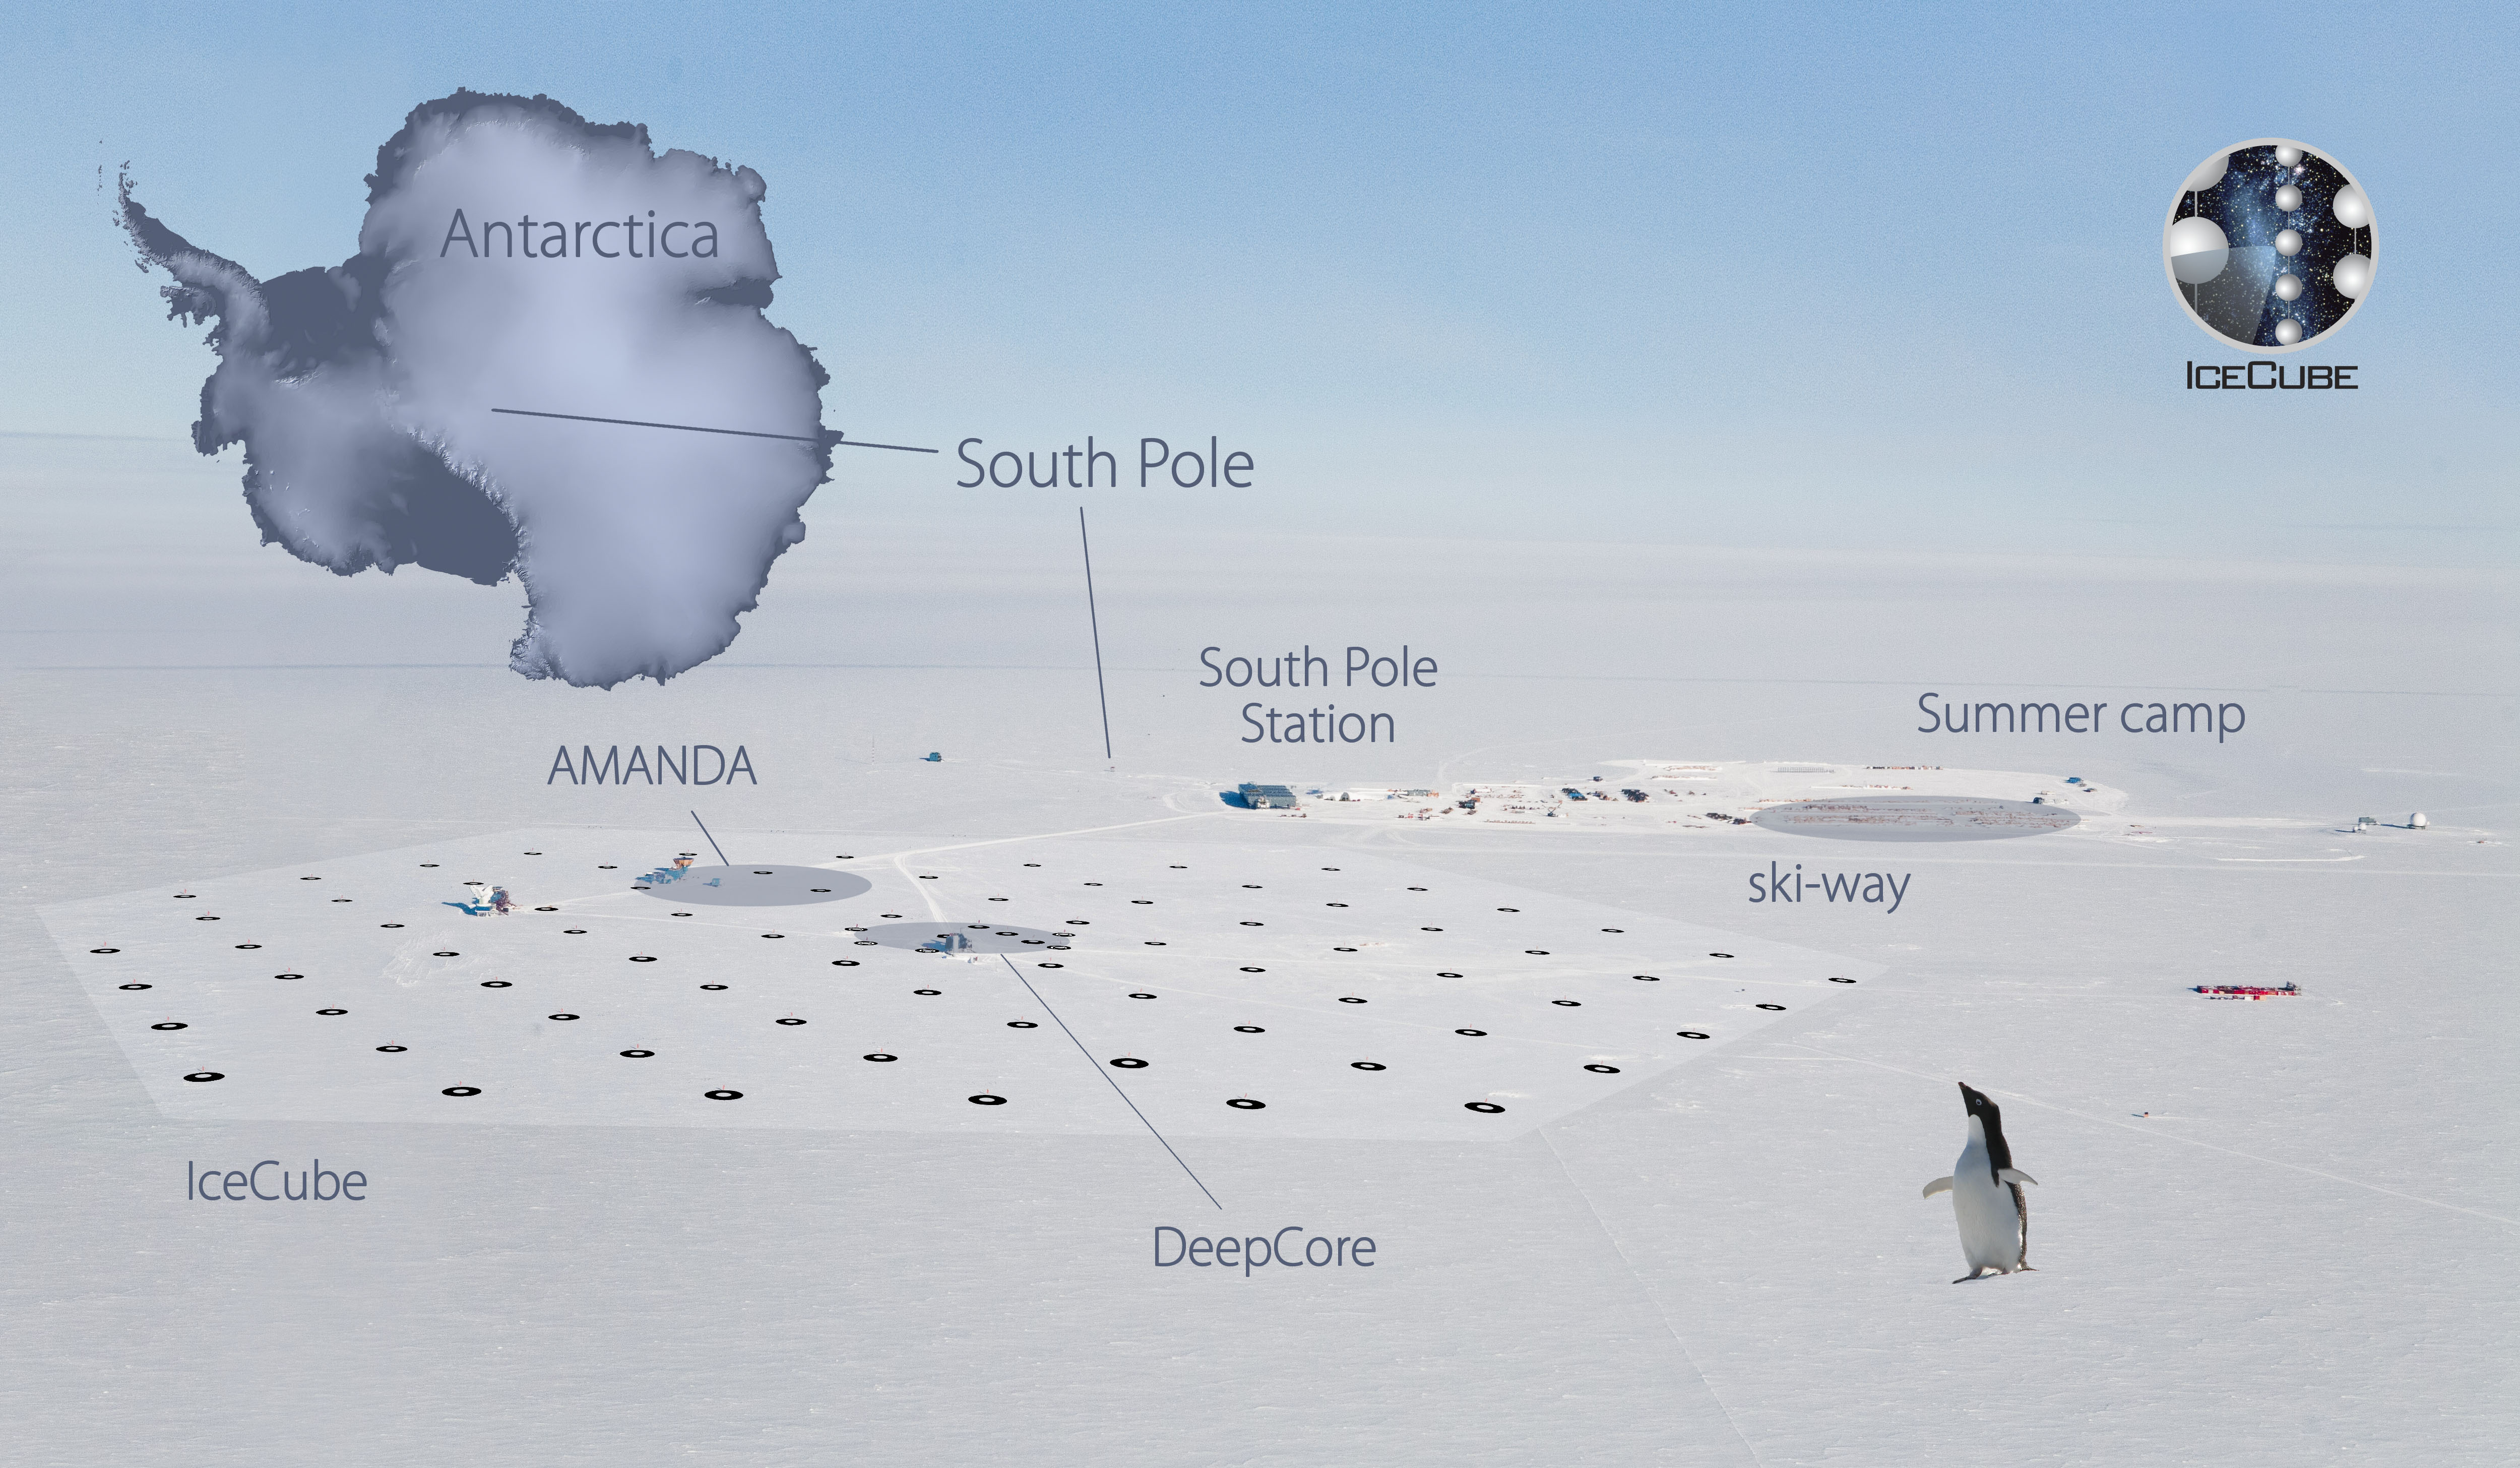
\includegraphics[keepaspectratio,height=14.5cm]{pole-view}
\end{center}

\Tr
\begin{center}
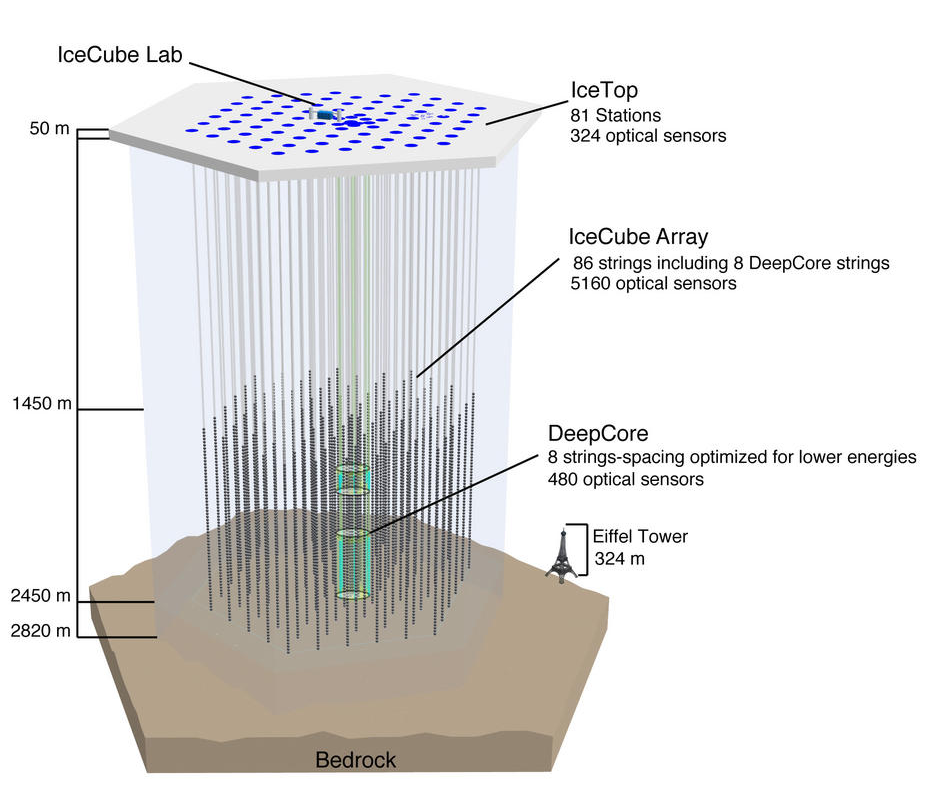
\includegraphics[keepaspectratio,height=14cm]{ic86-dc}
\end{center}

\Tr
\begin{center}
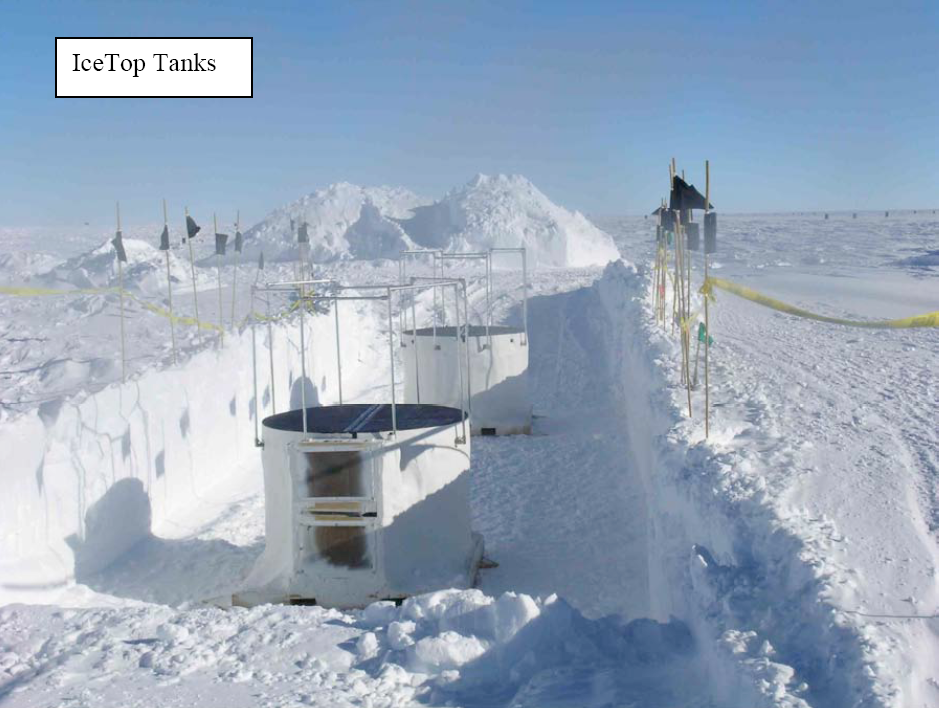
\includegraphics[keepaspectratio,height=14.5cm]{icetop-snow}
\end{center}

\Tr
\begin{center}
{\blue IceTop detectieprincipe}\\[5mm] 
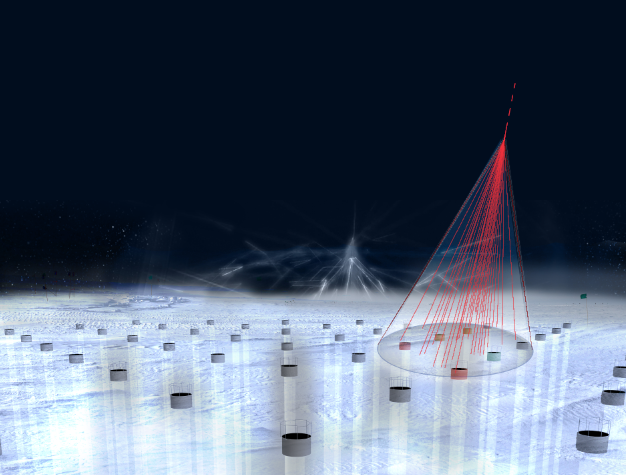
\includegraphics[keepaspectratio,height=14cm]{cr-shower2}
\end{center}

\Tr
\begin{center}
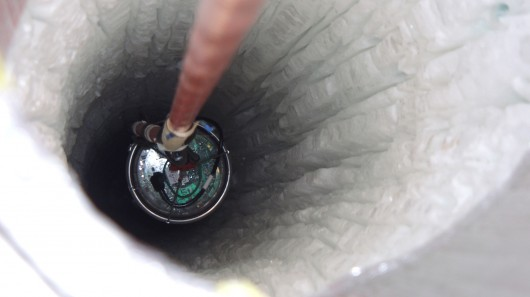
\includegraphics[keepaspectratio,height=14cm]{hole2}
\end{center}

\Tr
\twocolumn[\begin{center}{\blue InIce detectieprincipe}\end{center}]
\begin{center}
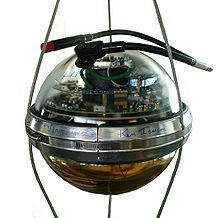
\includegraphics[keepaspectratio,height=6cm]{dom}\\[3mm]
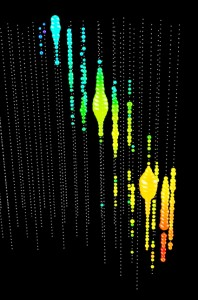
\includegraphics[keepaspectratio,height=7cm]{event}
\end{center}
%
\newpage
%
\begin{center}
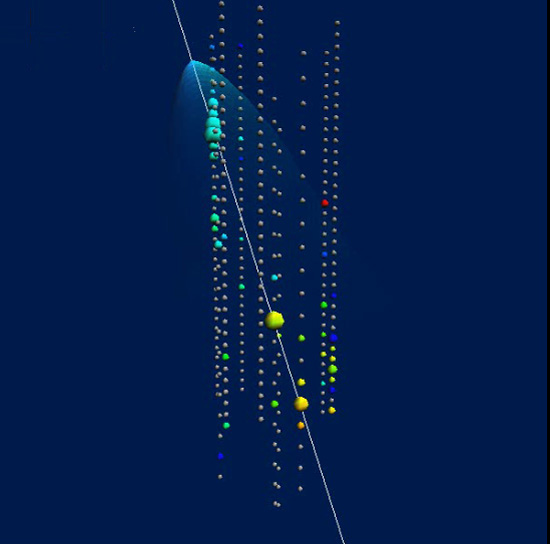
\includegraphics[keepaspectratio,width=13.5cm]{cone}
\end{center}

\Tr
\onecolumn
\begin{center}
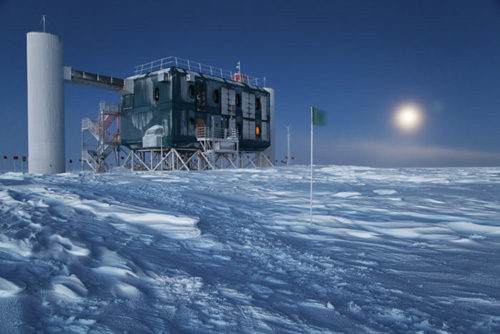
\includegraphics[keepaspectratio,height=14cm]{icl2}
\end{center}

\Tr
\onecolumn
\begin{center}
{\red Muonen van atmosferische interacties}\\[1cm]
{\blue De schaduw van de Maan}\\[5mm]
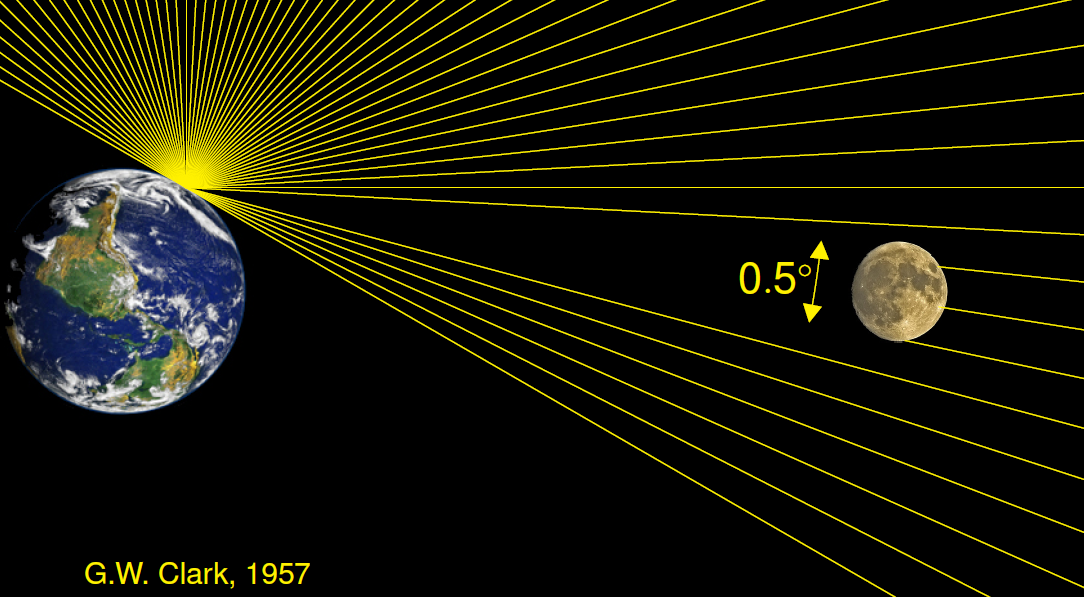
\includegraphics[keepaspectratio,height=8cm]{moon-shadow1}
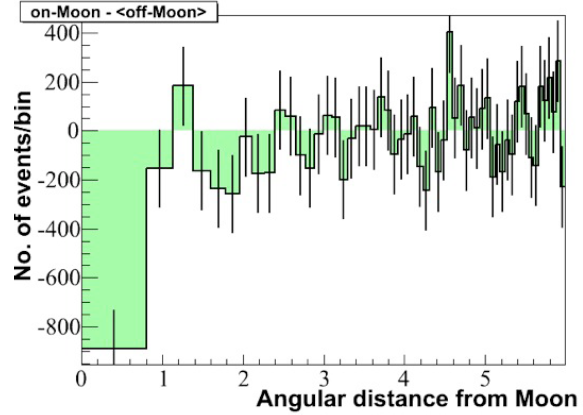
\includegraphics[keepaspectratio,height=8cm]{moon-shadow2}\\[1cm]
{\blue Hoekresolutie : $\sim 0.8^{\circ}$}
\end{center}

\Tr
\onecolumn
\begin{center}
{\blue De IceCube hemelkaart} (7 jaar data, $\sim$700'000 events)\\[5mm]
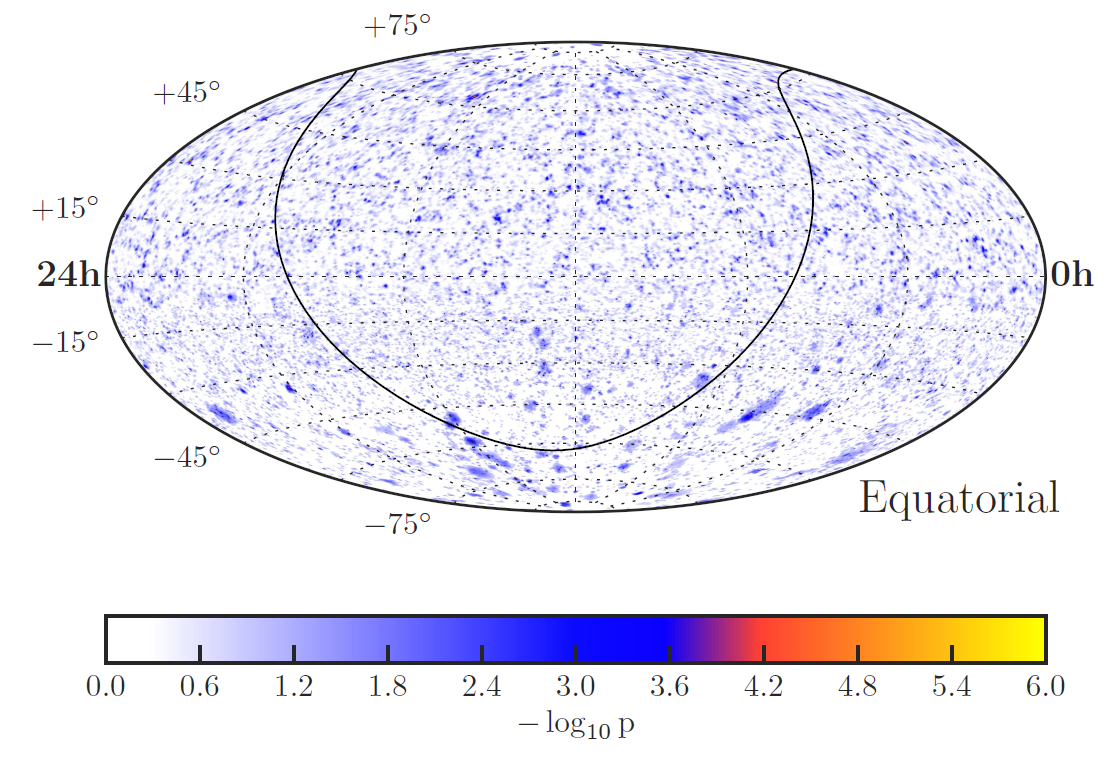
\includegraphics[keepaspectratio,height=14cm]{icecube-skymap-7years}
\end{center}
